\documentclass[11pt]{article}
\usepackage{geometry}
\geometry{letterpaper}

\usepackage{graphicx}
\usepackage{amssymb}
\usepackage{float}
\usepackage{tabularx}
\usepackage{multicol}
\usepackage{hyperref}
\hypersetup{
    colorlinks,
    citecolor=black,
    filecolor=blue,
    linkcolor=black,
    urlcolor=black
}

\begin{document}

\begin{titlepage}
	\newcommand{\HRule}{\rule{\linewidth}{0.2mm}}
	\begin{center}
	\textsc{\LARGE McMaster University}\\[1.5cm]

	\textsc{\Large SmartServe}\\[0.5cm]
	\textsc{\large Software \& Mechatronics Capstone}\\[0.5cm]

	\HRule\\[0.4cm]
		{\huge\bfseries Low Level System Design}\\[0.4cm]
	\HRule\\[0.4cm]

	\begin{minipage}[t][][t]{0.5\textwidth}
		\begin{flushleft} \large
			\emph{Authors:}\\
			Christopher McDonald\\
			Harit Patel \\
			Janak Patel \\
			Jared Rayner  \\
			Nisarg Patel  \\
			Sam Hamel \\
			Sharon Platkin \\
		\end{flushleft}
	\end{minipage}
	~
	\begin{minipage}[t][][t]{0.4\textwidth}
		\begin{flushright} \large
			\emph{Professor:} \\
			Dr. Alan Wassyng \\[0.4cm]
			\emph{Teaching Assistants:} \\
			Bennett Mackenzie \\
			Nicholas Annable \\
			Stephen Wynn-Williams \\
			Viktor Smirnov
		\end{flushright}
	\end{minipage}\\[2cm]

	
\includegraphics[width=0.3\textwidth]{../logo.png} \\
	{\large Last compiled on \today}
	\end{center}

\end{titlepage}

\tableofcontents
\listoffigures

\vfill
\begin{figure}[H]
   \centering
   \noindent\begin{tabularx}{\textwidth}{| >{\centering\arraybackslash}m{0.2\textwidth} | >{\centering\arraybackslash}m{0.2\textwidth} | >{\centering\arraybackslash}m{0.2\textwidth} | >{\centering\arraybackslash}m{0.285\textwidth} |}
   \hline
   \textbf{Date} & \textbf{Revision} & \textbf{Comments} & \textbf{Author(s)} \\ \hline
   Dec 29, 2017 & 1.0 & Structure made for document including headings & Christopher McDonald \\ \hline
   Jan 11, 2018 & 1.1 & Added content for ShotRecommendation and SmartServe systems, and Communication Protocols Sections & Christopher McDonald \\
   Jan 11, 2018 & 1.2 & Added content for Document Overview & Christopher McDonald \\ \hline
   Jan 12, 2018 & 1.3 & Added Data Storage and User Interface modules & Sharon Platkin \\ \hline
   Jan 13, 2018 & 1.4 & Added details for Shooting Mech, CV, Shot Optimizer, Shooting Model subsystems & Harit Patel \& Sam Hamel \\ \hline
   Jan 15, 2018 & 1.5 & Edited Module Guide & Sharon Platkin \\ \hline

   \end{tabularx}
   \caption{Revision History}
\end{figure}
\newpage
\section{Introduction}
\subsection{Project Overview}
SmartServe is an autonomous table tennis training system for table tennis players with various skill levels. SmartServe aids in diagnosing and improving a player's performance over time. The system trains table tennis players by shooting table tennis balls towards the player and detects successful returns from the player. The system can further adapt to the player's weaknesses and help them overcome it through further training. Importantly, SmartServe alleviates the problems of finding and working with a coach for players, as well as coaches trying to train multiple players simultaneously. The system will be deemed a success if the table tennis players and coaches can enjoy and see some value added by using SmartServe. \\\\
The project started at the beginning of the Fall 2017 academic term and will conclude at the end of the Winter 2018 term. In addition, the core project team consists of final year Software and Mechatronics Engineering students who are enrolled in the MECHTRON 4TB6/SFWRENG 4G06 capstone project course.
\subsection{Document Overview}
This document will add more detail into the subsystems introduced in the High-Level System Design document (HLSD) found \href{run:../Design.pdf}{here}. The HLSD omitted details such as how the subsystems would work, how they are built and how communication will be handled between them. This document will cover all of those details and introduce how each subsystem will be programmed by defining the language and libraries required. \\ \\
All software developers on the development team should read this document when building the subsystems to ensure the correct data is being sent and communication portals are set up correctly. Each subsystem will hold one to many modules and each module will contain one to many methods or variables. A detailed class diagram will organize all the subsystems and their modules with arrows indicating which module uses another one.
\subsection{Naming Conventions and Terminology}
\label{sec:definitions}
The following terms and definitions will be used throughout this document:
\begin{itemize}
% Alphabetical order is highly preferred as it eases user navigation
\item \textbf{ACID}: a database transaction which is atomic, consistent, isolated and durable
\item \textbf{ADT}: abstract data type
\item \textbf{CV}: computer vision
\item \textbf{FPS}: frames per second
\item \textbf{FSM}: finite state machine, shows transitions between states
\item \textbf{GUI}: graphical user interface
\item \textbf{IPO}: input process output
\item \textbf{Pitch}: rotation along the y-axis; this rotation angle primarily dictates the range of the ball from the net to the edge of the table on the user side
\item \textbf{Roll}: rotation along the x-axis
\item \textbf{Shooting Mechanism}: refers to the part of the system that shoots the table tennis balls towards the user side (player) Please refer to Figure \ref{fig:table-tennis-top-view} for visual illustration
\item \textbf{System}: encompasses both the hardware and software parts of SmartServe
\item \textbf{System Side}: the side of the table where the electromechanical system is placed; it is the opposite side of the User Side Please refer to Figure \ref{fig:table-tennis-top-view} for visual illustration
\item \textbf{TCP:} transmission control protocol
\item \textbf{Team}: all team members of the core capstone project, as noted in the list of Authors
\item \textbf{UI}: user interface
\item \textbf{User Side}: the side of the table where the user (player) is standing
\item \textbf{Yaw}: rotation along the z-axis; this rotation angle primarily dictates the panning functionality of the shooting mechanism from the right side to the left side of the table
\end{itemize}

\begin{figure}[H]
   \centering
   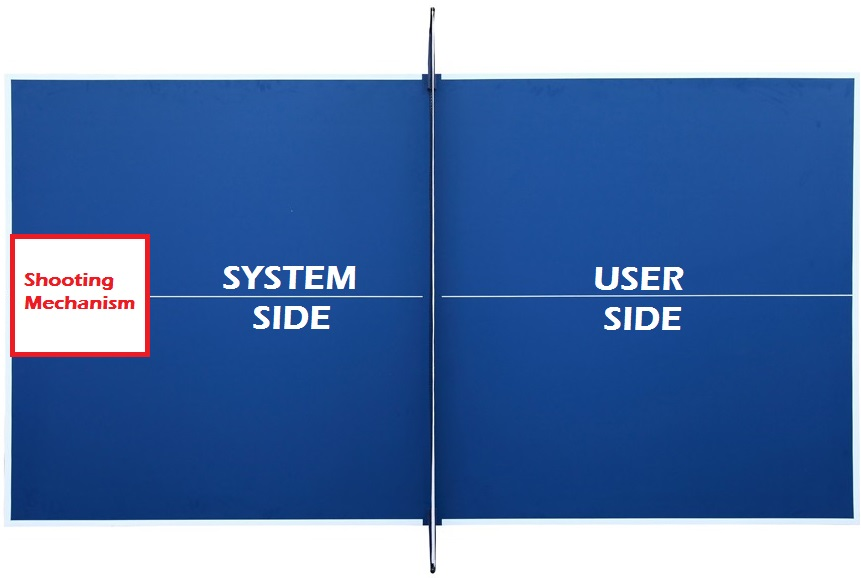
\includegraphics[width=0.75\textwidth]{../img/Table-Tennis-Top-View.png} %requires the graphicx package
   \caption{Top View of the Tennis Table}
   \label{fig:table-tennis-top-view}
\end{figure}

\section{Detailed Class Diagram}

\section{Module Guide}
\subsection{SmartServe Modules} % Chris - edited by Sharon
\subsubsection*{Controller}
\textbf{Responsibilities} \\
The controller handles all the timing constraints and sequential events for shooting balls towards the player. It is the interface for the UI to allow the user to preform any and all actions. \\ \\
\textbf{Secrets} \\
The sequence and timing constraints of the shooting procedure. \\ \\
\textbf{MID}
\begin{itemize}
\item \textbf{boot} - none \\ returns: \textit{boolean} \\ description: instantiates all dependancies and ensures services are working as expected
\item \textbf{startTraining} - Mode m \\ returns: \textit{boolean} \\ description: starts the shooting procedure given a certain training Mode
\item \textbf{stopTraining} - none \\ returns: \textit{boolean} \\ description: stops the training procedure
\item \textbf{setShootingParameters} - ShootingParameters sp \\ returns: \textit{boolean} \\ description: sets the shooting parameters for certain table sizes
\end{itemize}

\subsubsection*{ArduinoConnector}
\textbf{Responsibilities} \\
This module is responsible for facilitating the communication with the Arduino which is part of the Shooting Mechanism subsystem. This includes sending and receiving messages as well as ensuring proper testing of the connection is preformed. \\ \\
\textbf{Secrets} \\
The connection to the Arduino. \\ \\
\textbf{MID}
\begin{itemize}
\item \textbf{test} - int port \\ returns: \textit{boolean} \\ description: tests connection to the Arduino
\item \textbf{shoot} - float pitch, float yaw, float angularVelocity \\ returns: \textit{none} \\ description: instructs Arduino to shoot the ball in a certain way
\item \textbf{position} - none \\ returns: \textit{Position} \\ description: returns the position of the mechanism
\end{itemize}

\subsubsection*{ShotRecommendationConnector}
\textbf{Responsibilities} \\
This module is responsible for facilitating the communication with the Shot Recommender subsystem. This includes sending and receiving messages as well as ensuring proper testing of the connection is preformed. \\ \\
\textbf{Secrets} \\
The connection to the Shot Recommender. \\ \\
\textbf{MID}
\begin{itemize}
\item \textbf{connect} - int port, [optional] String ip \\ returns: \textit{boolean} \\ description: instantiates all dependancies and ensures services are working as expected
\item \textbf{getRecommendation} - none \\ returns: \textit{Shot} \\ description: returns the shot data to shoot towards the player

\item \textbf{updateModel} - Shot shot, boolean returned \\ returns: \textit{none} \\ description: sends data to ShotRecommender on whether a shot was returned or not
\end{itemize}

\subsubsection*{CVConnector}
\textbf{Responsibilities} \\
This module is responsible for facilitating the communication with the CV (Computer Vision) subsystem. This includes sending and receiving messages as well as ensuring proper testing of the connection is preformed. \\ \\
\textbf{Secrets} \\
The connection to the CV system. \\ \\
\textbf{MID}
\begin{itemize}
\item \textbf{connect} - int port \\ returns: \textit{boolean} \\ description: tests connection to CV subsystem
\item \textbf{start} - none \\ returns: \textit{boolean} \\ description: instructs CV to begin tracking and return data for shot

\end{itemize}

\subsubsection*{SQLConnector}
\textbf{Responsibilities} \\
This module is responsible for facilitating the communication with the Data Storage subsystem. This includes sending and receiving messages as well as ensuring proper testing of the connection is preformed. \\ \\
\textbf{Secrets} \\
The connection to the Data Storage system. \\ \\
\textbf{MID}
\begin{itemize}
\item \textbf{connect} - int port, [optional] String ip \\ returns: \textit{boolean} \\ description: tests connection to Data Storage subsystem on port \textit{port} at the IP Address \textit{ip} or \textit{localhost} if ip is unavailable
\item \textbf{query} - String procedure, Map<String, String> values \\ returns: \textit{ResultSet} \\ description: returns data from database based on procedure ran and values given
\item \textbf{save} - String procedure, Map<String, String> values \\ returns: \textit{boolean} \\ description: returns success information on write to database based on procedure ran and values given
\end{itemize}

\subsection{Shot Recommendation Modules} % Chris - edited by Sharon
\subsubsection*{Controller}
\textbf{Responsibilities} \\
This module will act as the API interface for the Shot Recommendation subsystem. As such, it will accept requests and return the appropriate data. It will also communicate will other modules should a user of this system need to do so. \\ \\
\textbf{Secrets} \\
The process for handling Shot Recommendation requests. \\ \\
\textbf{MID}
\begin{itemize}
\item \textbf{listen} - none \\ returns: \textit{none} \\ description: waits for a request made for a shot
\item \textbf{query} - String procedure,  dict values, [optional] int port, [optional] String ip \\ returns: \textit{Cursor} \\ description: gets data from a stored procedure using some set of values for a MySQL instance on port \textit{port} at the IP Address \textit{ip}
\end{itemize}

\subsubsection*{Model}
\textbf{Responsibilities} \\
This module will hold the data for each user in such a way information can be extracted. It will contain an internal model which is built from the data and use it to recommend a new shot. \\ \\
\textbf{Secrets} \\
The algorithm to build the model. \\ \\
\textbf{MID}
\begin{itemize}
\item Model \textbf{model} - representation of shot performance data for extracting information
\item \textbf{train} - Cursor cur \\ returns: \textit{none} \\ description: using some data from Cursor, this will train the model
\item \textbf{next} - none \\ returns: \textit{Shot} \\ description: returns a shot based on the user's past performance
\end{itemize}

\subsection{Shooting Model Modules}
\subsubsection*{Shot}
\textbf{Responsibilities} \\
Specific details (such as yaw and speed) that are required to take the desired shot are stored within this abstract data type module. \\ \\
\textbf{Secrets} \\ 
None \\  \\
\textbf{MID} 
\begin{itemize}
\item \textbf{shot} - double yaw, double velocity \\ returns: \textit{none} \\ description: constructor to store the shooting model details in an abstract data type.
\item \textbf{toString} - none \\ returns: \textit{String} \\ description: Returns shooting details in a printable string format.
\end{itemize}

\subsubsection*{Shooting Model}
\textbf{Responsibilities} \\
Responsible for mapping a desired shot to the details needed to take the shot. \\ \\
\textbf{Secrets} \\ 
Methods and formulas being used to identify the required details needed to take the desired shot. \\  \\
\textbf{MID} 
\begin{itemize}
\item \textbf{shootingModel} - double  initialHeight, double xInitialHeight, double pitch \\ returns: \textit{none} \\ description: instantiates the shooting model subsystem.
\item \textbf{getShotDetails} - double landingXCoord, double landingYCoord \\ returns: \textit{Shot} \\ description: calculates details to take the desired shot and stores them within the ADT.
\end{itemize}

\subsection{Shot Optimizer Modules}
\subsubsection*{Controller}
\textbf{Responsibilities} \\
This module is responsible for facilitating the communication with the Shot Optimizer system. This includes sending and receiving messages as well as ensuring proper testing of the connection is performed. \\ \\
\textbf{Secrets} \\ 
The connection to the Shot Optimizer system. \\ \\
\textbf{MID} 
\begin{itemize}
\item \textbf{connect} - int  port, [optional] String ip \\ returns: \textit{boolean} \\ description: instantiates all dependancies and ensures services are working as expected.
\item \textbf{getOrientation} - Position  position \\ returns: \textit{Orientation} \\ description: returns the optimal orientation data to orient the shooting mechanism.
\end{itemize}

\subsection{Computer Vision Modules}
\subsubsection*{Detect}
\textbf{Responsibilities} \\
This module detects successful returns from the user, and sends that data to smartserve\\
\textbf{Secrets} \\ 
Success criteria of returns and how the camera feed is analyzed.\\ 
\textbf{MID} 
\begin{itemize}
\item \textbf{Detect} - Camera Capture cap \\ returns: \textit{none} \\ description: Detects if the ball was succesfully returned by the user and calls the Send function
\item \textbf{Send} -  none \\ returns: \textit{none} \\ description: Sends a signal to Smartserve indicating that a successful return was made
\end{itemize}

\subsection{Data Storage Modules}
\subsubsection*{Global}
\textbf{Responsibilities} \\
Communicates with the database to create, delete and update rows in various tables.  \\
\textbf{Secrets} \\
All connection information between the sub-systems, table contents.\\
\textbf{MID} \\
\begin{itemize}
\item User \textbf{user} - String user\textunderscore name, String password, int user\textunderscore id \\ description: representation of a user
\item Shot \textbf{shotType} - int zone\textunderscore id, int omega\textunderscore id, int shot\textunderscore id \\ description: representation of a shot type
\item Zone \textbf{user} -  int zone\textunderscore id, double x\textunderscore loc, double y\textunderscore loc \\ description: representation of a zone on the table, used as a look up table
\item Omega \textbf{user} - int omega\textunderscore id, double angle, double velocity \\ description: representation of angular velocity of the ball, used as a look up table
\item ReturnRate \textbf{return\textunderscore rate} - int user\textunderscore id, int shot\textunderscore id,  Timestamp timeStamp, boolean returned \\ description: return statistics for each user
\item \textbf{signUp} - String userName, String password \\ returns: \textit{none} \\ description: adds a user row to the \textit{User} table
\item \textbf{nextShot} - int zone \\ returns: \textit{Shot} \\ description: determines which shot type to perform
\item \textbf{returned} - Timestamp timeStamp, User user, Shot shot \\ returns: \textit{none} \\ description: updates returnRate table for user for performance statistics
\end{itemize}

\subsection{Shooting Mechanism Modules}
This module will be specified in the hardware component design of the shooting mechanism.
\subsection{User Interface Modules}
\subsubsection*{Controller}
\textbf{Responsibilities} \\
Responsible for translating the desired action of the user from the View module to the SmartServe module. \\ \\
\textbf{Secrets} \\
Connection between modules and sub-systems. \\ \\
\textbf{MID}
\begin{itemize}
\item \textbf{main} - String args[] \\ returns: \textit{none} \\ description: calls the View module to initialize the UI
\item \textbf{setTrainingMode} - Mode m \\ returns: \textit{none} \\ description: sets mode from View module and sends it to SmartServe
\item \textbf{setShootingParameters} - none \\ returns: \textit{ShootingParameters} \\ description: sets shooting parameters from View module and sends it to SmartServe
\item \textbf{setStatistics} - none \\ returns: \textit{StatisticsParameters} \\ description: sets statistics parameters and sends them to View module
\item \textbf{signUp} - User user \\ returns \textit{none} \\ description: gets user information from view module and sends it to smartServe
\item \textbf{login} - User user \\ returns \textit{boolean} \\ description: gets user name and password from the View module and authenticates by calling SmartServe
\end{itemize}
\subsubsection*{View}
\textbf{Responsibilities} \\
The view module will contain all the actual visual aspects of the system that the user will interact with. This includes text, pictures, buttons, etc. \\ \\
\textbf{Secrets} \\
The structure and implementation of the view. \\ \\
\textbf{MID}
\begin{itemize}
\item \textbf{start} - none \\ returns: \textit{none} \\ description: general user interface code, called to initiate UI
\item \textbf{selectMode} - MouseEvent me\\ returns: \textit{Mode} \\ description: listens for a mouse click on mode types, and returns that mode
\item \textbf{calibrate} - none \\ returns: \textit{ShootingParameters} \\ description: collects user input for table size in order to calibrate the system
\item \textbf{startTrainingBtn} - MouseEvent me \\ returns: \textit{boolean} \\ description: listens for mouse click on start training button
\item \textbf{stopTrainingBtn} - MouseEvent me \\ returns: \textit{boolean} \\ description: listens for mouse click on stop training button
\item \textbf{viewStatsBtn} - MouseEvent me \\ returns: \textit{none} \\ description: listens for mouse click on statistics button and displays statistics to the user
\item \textbf{signUpBtn} - MouseEvent me \\ returns: \textit{User} \\ description: listens for mouse click on sign up button and collects user information
\item \textbf{loginBtn} - MouseEvent me \\ returns: \textit{User} \\ description: listens for mouse click on sign in button and displays profile if authenticated properly
\end{itemize}

\section{Communication Protocols} % Chris
\subsection{Smart Serve to Shot Recommendation}
The Shot Recommendation system (SR) will use Python to leverage machine learning libraries like SciKit Learn and the Smart Serve system (SS) will be implemented in Java. In order for the SS to communicate to the SR, it will make an HTTP request with some data and receive an HTTP response encoded using JSON. This allows the use of a reliable means of communication and flexibility to host the SR remotely if need be. \\ \\
The SS will make a GET request to the SR for requesting a shot to use and can make POST request to give data regarding whether a shot was returned or not. In the event the HTTP request takes too long, the SS should handle it accordingly by timing out and using random shots or continuing the program. \\ \\
HTTP libraries are standard in Java and a microframework for handling HTTP requests can be used for Python like \href{http://flask.pocoo.org}{flask}.
\subsection{Smart Serve to Shooting Mechanism}
The Shooting Mechanism system (SM) will implement an interface using an Arduino. The SS will use libraries for communicating to the Arduino to communicate to the SM which can be found \href{http://fizzed.com/oss/rxtx-for-java}{here} for 64-bit Windows and Linux installations and \href{http://blog.iharder.net/2009/08/18/rxtx-java-6-and-librxtxserial-jnilib-on-intel-mac-os-x/}{here} for 64-bit macOS installations. The SS does not need a response from the system, as it will tell the SM where to shoot and how to do so but does not need a response.
\subsection{Smart Serve to Computer Vision}
The SS will communicate to the Computer Vision subsystem (CV) via sockets over the TCP protocol using the Java Networking libraries and the Python socket libraries. The SS will initiate the communication to start tracking and expect a return value based on whether it was returned or not. The SS will timeout in the event the CV does not return a value after 1.5 seconds.
\subsection{Smart Serve to User Interface}
% probably pretty standard, using Swing or something
The SS and the User Interface system (UI) will both be programmed using Java. The UI system can interface with the SS by calling exposed public methods based on user input.
\subsection{Smart Serve to Shot Optimizer}
The SS and the Shot Optimizer system (SO) will both be programmed using Java. The SS system can interface with the SO by calling exposed public methods based on user input.
\subsection{Smart Serve to Shooting Model}
The SS and the Shooting Model system (SModel) will both be programmed using Java. The SS system can interface with the SModel by calling exposed public methods based on user input.
\subsection{Smart Serve to Data Storage}
The SS is programmed in Java and the Data Storage system (DS) will be implemented using Stored Procedures held in a MySQL database instance. In order for the SS to use the DS, a \href{https://dev.mysql.com/downloads/connector/j/5.1.html}{SQLConnector} can be used to do so.
\subsection{Shot Recommendation to Data Storage}
The SR is programmed in Python and the Data Storage system (DS) will be implemented using Stored Procedures held in a MySQL database instance. In order for the SR to use the DS, a \href{https://dev.mysql.com/doc/connector-python/en/}{SQLConnector} can be used to do so.




\end{document}
